%! suppress = MissingImport
This paragraph applies only to 2-lead pushbuttons:
\begin{quote}
    If your momentary pushbuttons are attached to a cardboard strip with tape, remove them from the cardboard strip.
    If your momentary pushbuttons' leads have metal tabs at the end (Figure~\ref{fig:pushbutton-tabs}), you will need to snip off the tabs before inserting the pushbutton leads into the breadboard;
    ordinary scissors will suffice for this task.
    Regardless of whether the leads have metal tabs at the end, you may optionally trim the leads to be about $\frac{1}{4}$in (6.4mm) long -- you can use the exposed lead from a jumper wire as a reference -- so that the pushbuttons sit flush on the breadboard.
    It is not necessary that they sit flush;
    this is simply to keep the buttons from wiggling under your fingers.
    \textit{Do not cut the leads shorter than $\mathit{\frac{1}{8}}$in (3.2mm)!}
    \textbf{Be sure to use eye protection in case the leads' ends fly off when you snip them.}
\end{quote}

This paragraph applies only to 4-prong pushbuttons:
\begin{quote}
    The four prongs on a momentary pushbutton are electrically connected as two pairs.
    If you attach the pushbuttons in the wrong orientation, it will appear to the \developmentboard as though they are always pressed.
    Fortunately, there is only one orientation that will place the prongs in the specified contact points.
    As long as the prongs are in the specified contact points, your pushbuttons will work fine.
    %TODO: add annotated photo of 4-prong electrical connections
\end{quote}

These are ``normally open'' momentary ``switches'' that close when pressed and re-open when released.
We will wire the pushbuttons such that they normally produce a 1, and when pressed will produce a 0.
Figure~\ref{fig:pushbutton-diagram} shows a diagram of the wiring for the pushbuttons.

\begin{figure}
    \centering
    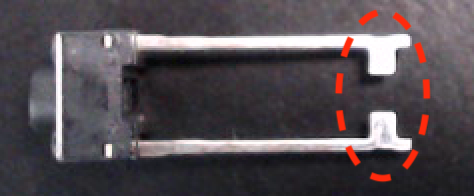
\includegraphics[height=2cm]{direct/buttons/pushbutton-tabs}
    \caption{Some momentary pushbuttons have metal tabs on their leads.\label{fig:pushbutton-tabs}}
\end{figure}

\begin{figure}
    \centering
    \subfloat[2-lead pushbuttons]{
        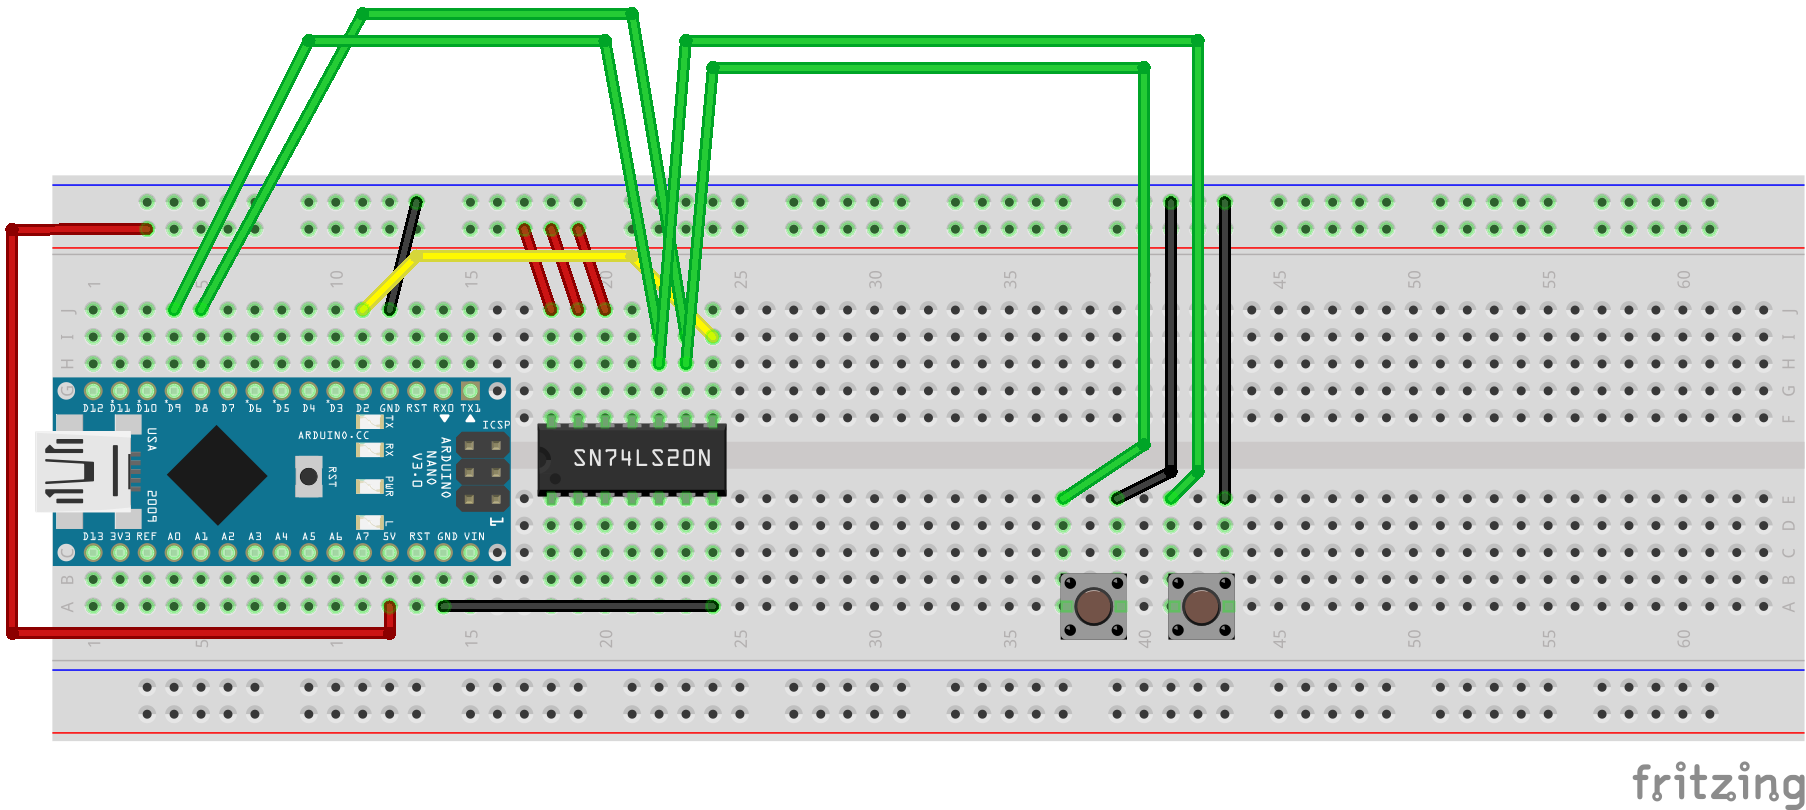
\includegraphics[width=0.9\textwidth]{fritzing_diagrams/pushbutton-2lead}
    }
    \hfil
    \subfloat[4-prong pushbuttons]{
        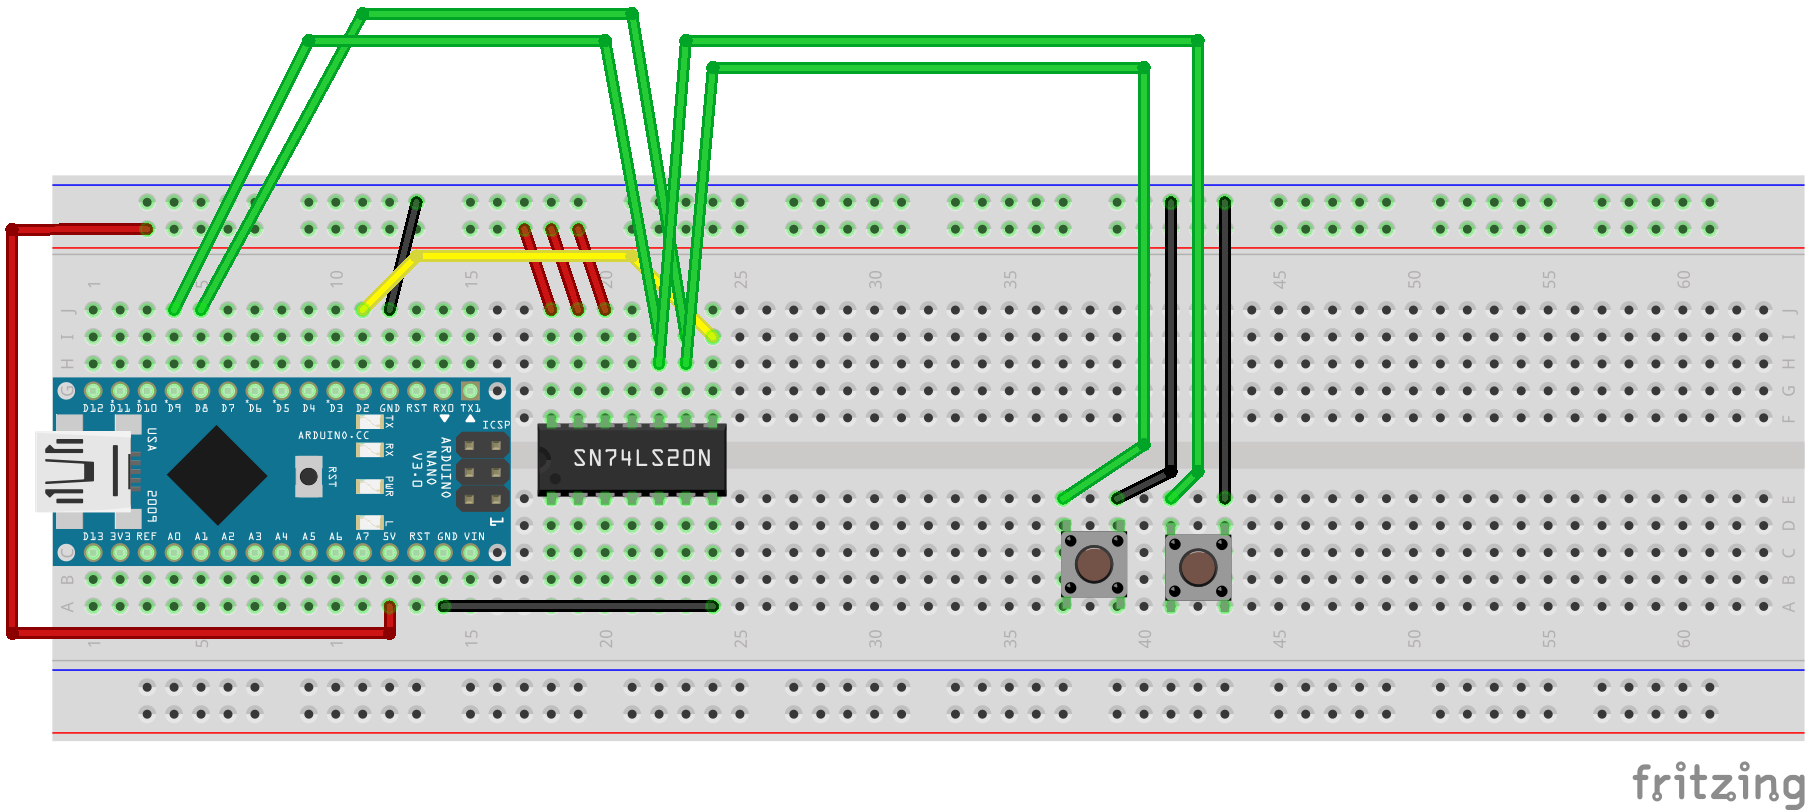
\includegraphics[width=0.9\textwidth]{fritzing_diagrams/pushbutton-4prong}
    }
    \caption{Diagram of wiring associated with momentary pushbutton input.
        \textit{Note: connection between the 74LS20's pin 7 and the \developmentboard's
        \mcubuttonnand\ pin was previously installed in Section~\ref{subsec:nand}.}
        \label{fig:pushbutton-diagram}}
\end{figure}

\disconnect\

\prepunch{a\controlrow{11}, a\controlrow{13}, a\controlrow{15}, and a\controlrow{17}}
If you have 4-prong pushbuttons, then also pre-punch holes into contact points d\controlrow{11}, d\controlrow{13}, d\controlrow{15}, and d\controlrow{17}.

If you have 2-lead pushbuttons:
\begin{quote}
    Insert the leads of one pushbutton into contact points a\controlrow{11} and a\controlrow{13}.
    Insert the leads of the other pushbutton into contact points a\controlrow{15} and a\controlrow{17}.
\end{quote}

If you have 4-prong pushbuttons:
\begin{quote}
    Insert the prongs of one pushbutton into contact points a\controlrow{11}, d\controlrow{11}, a\controlrow{13} and d\controlrow{13}.
    Insert the prongs of the other pushbutton into contact points a\controlrow{15}, d\controlrow{15}, a\controlrow{17} and d\controlrow{17}.
\end{quote}

Peel off one wire from the \rainbow, and use it to connect contact point e\controlrow{13} to the upper \ground.
Peel off one wire from the \rainbow, and use it to connect contact point e\controlrow{17} to the upper \ground.

Use two wires from the \rainbow to connect the ungrounded side of the left pushbutton to the 74LS20 and to the \developmentboard:
connect e\controlrow{11} to \leftbuttontarget, and connect \mculeftbuttonfrom\ to \mculeftbuttonpoint.
Now use another two wires from the \rainbow to connect the ungrounded side of the right pushbutton to the 74LS20 and to the \developmentboard:
connect e\controlrow{15} to \rightbuttontarget, and connect \mcurightbuttonfrom\ to \mcurightbuttonpoint.
\textit{Notice that there are no wires in \nanduppernc} because, as you can see in Figure~\ref{fig:nand-pinout}, the 74LS20's pin 11 is not connected (``NC'') to anything.

See Figure~\ref{fig:pushbutton-wired}.

\begin{figure}%\begin{multicols}{2}
    \centering
    \subfloat[The momentary pushbuttons, wired to the 74LS20 and the \developmentboard.]{
        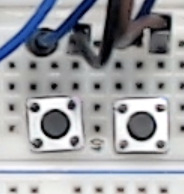
\includegraphics[height=4cm]{direct/buttons/pushbutton-2lead}
    }
%    \columnbreak
%
%    \subfloat[Connections between the momentary pushbuttons and the 74LS20.]{
%        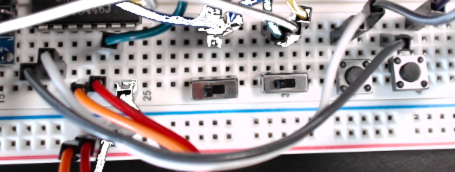
\includegraphics[width=0.55\textwidth]{direct/buttons/pushbutton-nand}
%        \label{fig:pushbutton-nand}
%    }
%
%    \subfloat[Connections between the \developmentboard\ and wiring to the momentary
%        pushbuttons.]{
%        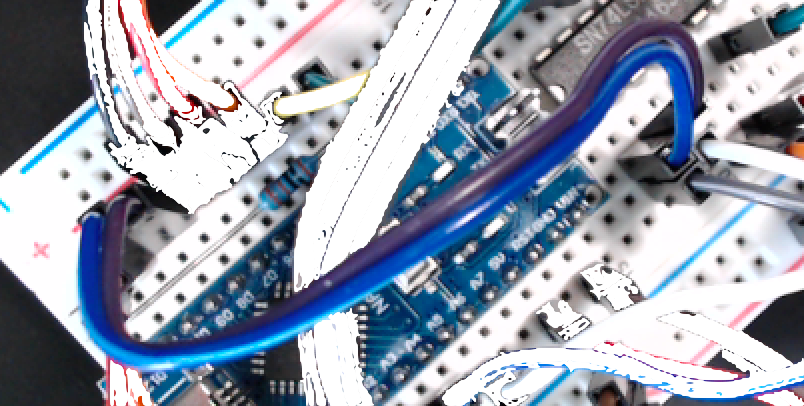
\includegraphics[width=.55\textwidth]{direct/buttons/pushbutton-nano}
%        \label{fig:pushbutton-nano}
%    }
%    \end{multicols}
    \caption{Wiring the Momentary Pushbuttons.
        \label{fig:pushbutton-wired}}
\end{figure}

When you have finished setting up the pushbuttons' wiring, there should be the electrical paths described in Table~\ref{tab:pushbutton}.

\begin{table}
    \begin{center}\begin{tabular}{||c|c|c|c||} \hline\hline
    Pushbutton                      & 74LS20                & \developmentboard\ pin    & Pulled High/Low \\ \hline
    Left button's grounded lead     &                       &                   & Pulled Low    \\
    Left button's ungrounded lead   & Upper NAND Input      & \mculeftbutton    &               \\
    Right button's grounded lead    &                       &                   & Pulled Low    \\
    Right button's ungrounded lead  & Upper NAND Input      & \mcurightbutton   &               \\
                                    & Upper NAND Input      &                   & Pulled High   \\
                                    & Upper NAND Input      &                   & Pulled High   \\
                                    & Upper NAND Output     & \mcubuttonnand    &               \\ \hline
                                    & pin 11 (\nanduppernc) & \multicolumn{2}{c||}{not connected / floating} \\ \hline\hline
    \end{tabular}\end{center}
    \caption{Electrical Paths for Momentary Pushbuttons.\label{tab:pushbutton}}
\end{table}

\checkpoint{inserted and wired the momentary pushbuttons}

%TODO: update for library examples
Connect your \developmentboard\ to the computer.
In the IDE's Serial Monitor, notice that the LEFT~BUTTON is always 1, the RIGHT~BUTTON is always 1, and the BUTTON~NAND is always 0.
Notice that when you press a button, the Serial Monitor shows that its value becomes 0, and when you release a button, its value becomes 1 again.
If either button is pressed, BUTTON~NAND becomes 1, and it is 0 only when both buttons are not pressed.